\chapter{Models}
\label{sec:models}

This chapter explores different probabilistic models for the problem, explains how they can be efficiently learned from data and presents the learning algorithm performance on synthetic data.

\section{Submodular model: FLID}

The Facility Location Diversity (FLID) model was first proposed in \cite{tschiatschek16learning} and belongs to the class of log-submodular probability distributions over sets.

\begin{definition}
  A distribution over sets $S \subseteq V$, where w.l.o.g $V = \{1,\dots,|V|\}$, of the form $P(S) = \frac{1}{Z}\mathrm{exp}(F(S))$ is called a log-submodular probability distribution, if $F(S)$ is a submodular function \cite{djolonga14variational}.
\end{definition}

\begin{definition}
  \label{def:submodularity}
  A function $F:2^V \rightarrow \mathbb{R}$ is submodular if it exhibits a "diminishing returns" property \cite{krause14submodular}, namely:
    \begin{equation*}
      \forall S,T \subseteq V : S \subseteq T, i \notin T \mid F(S \cup i) - F(S) \geq F(T \cup i) - F(T)
    \end{equation*}
\end{definition}

Submodular functions intuitively indicate that adding an item to a smaller set results in a larger gain than adding it to a larger one. This is a natural property in the context of summarization where adding more information to a large summary is less effective than adding it to a smaller one.

The FLID model consists of two terms, first a modular one which considers the utility or relevance of the items in the set, namely:

\begin{equation}
  P(S) \propto \exp\left(\sum_{i \in S}u_{i}\right)
\end{equation}

Where $u_{i} \in \mathbb{R}$ quantifies the utility of item $i$. In the context of location summarization, this utility could be proportional to the popularity of a place and how many times it has been photographed.

The diversity term is based on the idea of a latent concept space of dimension $L$ where each item can be represented with a vector $\mathbf{w}^{D}_{i} \in \mathbb{R}^{L}_{\geq 0}$. The representation in this space allows the model to identify items that are similar and penalize sets that include them together. Formally, the diversity term for a set $S \subseteq V$ is:

\begin{equation}
  \label{eq:diversity}
  \mathrm{div}(S) = \sum_{d=1}^{L}\left(\max_{i \in S}{w^{D}_{i, d}} - \sum_{i \in S}{w^{D}_{i,d}}\right)
\end{equation}

Putting this two terms together results in the \ref{eq:flid} probability model proposed in \cite{tschiatschek16learning}.

\begin{equation}
  \tag{FLID}
  P(S) = \frac{1}{Z}\exp{\left(\sum_{i \in S}u_{i} + \sum_{d=1}^{L}\left(\max_{i \in S}{w^{D}_{i, d}} - \sum_{i \in S}{w^{D}_{i,d}}\right)\right)}
  \label{eq:flid}
\end{equation}

In this model, $\mathbf{u} \in \mathbb{R}^{|V|}$ is the vector of utilities and $\mathbf{W}^{D} \in \mathbb{R}_{\geq 0}^{|V| \times L}$ is the diversity weight matrix where each row is the aforementioned $\mathbf{w}^{D}_{i}$ vector.

\subsection{Partition function}

In log-submodular probabilistic models, the normalization constant $Z$ is known as the \textit{partition function} \cite{djolonga14variational} and its exact computation is known to be \#P-complete \cite{jerrum1990}.  However, it has been proven \cite{tschiatschek16learning} that for FLID the partition function can be computed exactly in $\mathcal{O}(|V|^L)$ time, which can be efficient for $L \ll |V|$. This is an important property because the partition function is necessary to compute marginal probabilities and other quantities.

\subsection{Example: Two landmarks}
\label{sec:flid-toy}

In order to illustrate the model, consider a town with 3 popular locations: A town hall ($h$), a statue ($s$) and a fountain ($f$). Data shows that visitors only take photos at the town hall and the statue, or at the town hall and the fountain. This can be modeled with FLID, introducing a latent concept that discourages taking photos of both the fountain and statue.

Concretely, let $V = \{h, s, f\}$ and $\mathbf{u} = \left(2, 2, 2\right)$, indicating that all locations are equally popular. A suitable diversity weight vector would then be $\mathbf{W}^{D} = \left(0, 20, 20\right)^{\intercal}$. Table \ref{tab:flid-toy-probs} shows the resulting probabilities of the subsets, accurately representing the aforementioned description of the problem.

\begin{table}
  \centering
  \caption{FLID probability distribution for the scenario in example \ref{sec:flid-toy}}
  \begin{tabular}{@{}ll@{}}
    \toprule
      $S$ & $P(S)$  \\
    \midrule
      $\{h,s\}, \{h,f\}$ & $\approx 0.41$ \\
      $\{h\}, \{s\}, \{f\}$ & $\approx 0.06$ \\
      $\{\}, \{s,f\}, \{h,s,f\}$ & $\approx 0.00$ \\
    \bottomrule
  \end{tabular}
  \label{tab:flid-toy-probs}
\end{table}

\section{Mixed model: FLDC}

Diversity is an important property in the context of summarization \cite{tschiatschek16learning}, however coherence is also a desired property of summaries, especially in the context of structured timeline summarization \cite{Yan:2011:ETS:2009916.2010016}. Balancing coherence and diversity is considered a challenge because maxiziming only one of these properties may lead to poor results on the other one \cite{Shahaf2012}.

In order to model coherence in this model, the addition of a log-supermodular term analogous to the diversity term \ref{eq:diversity} is proposed.

\begin{definition}
  \label{def:supermodularity}
  A function $F:2^V \rightarrow \mathbb{R}$ is supermodular iff $-F(S)$ is submodular.
\end{definition}

The supermodular term encodes the items into another latent concept space, of dimension $K$, where sets containing items with high values in some latent dimension are rewarded. Hence modeling complementarity between items.

Concretely, consider a spatial summary of a city where people tend to stay close to the city center. A possible latent dimension could encode the distance to the center, and rewarding coherence on this dimension would create summarizes where all locations are close together which is the modeled behavior.

The extended model will be reffered to as the Facility Location Diversity and Coherence (\ref{eq:fldc}) model and its probability distribution is:

\begin{equation}
  \tag{FLDC}
  P(S) = \frac{1}{Z}\exp{\left(\sum_{i \in S}{u_{i}} + \mathrm{div}(S) + \sum_{c=1}^{K}{\left(\sum_{i \in S}{w^{C}_{i,c}} - \max_{i \in S}{w^{C}_{i,c}}\right)}\right)}
  \label{eq:fldc}
\end{equation}

Where $\mathbf{w}_{i}^{C}$ is the $i$-th row of the $\mathbf{W}^{C} \in \mathbb{R}_{\geq 0}^{|V| \times K}$ matrix and corresponds to the representation of item $i$ in the concept space of dimension $K$.

It should be noted that the FLDC model is neither log-submodular or log-supermodular unless $K=0$ or $L=0$, respectively. However, it can be used and learned in a similar fashion as the FLID model.

\subsection{Example: Disjoint pairs}
\label{sec:fldc-toy}

As an example of the extended model, consider the distribution presented in table \ref{tab:fldc-toy-probs} for $V = \{1,2,3,4\}$. It represents a set of two disjoint pairs, which indicates there exists a diversity component between the two pairs whilist having a coherence component between the items contained in each pair.

Concretely, the weight matrices $\mathbf{W}^{D}, \mathbf{W}^{C}$ in figure \ref{fig:fldc-toy-mixed-weights} illustrate one possible instance of the model. The corresponding utility vector is $\mathbf{u} = \overrightarrow{0}$, because there is no indication that individual items are favored over the pairs. Note that this model is easily interpretable and accurately realizes the distribution.

\begin{table}
  \centering
  \caption{Probability distribution for example \ref{sec:fldc-toy}}
  \begin{tabular}{@{}ll@{}}
    \toprule
    $S$ & $P(S)$  \\
    \midrule
    $\{1,2\}, \{3,4\}$ & $0.5$ \\
    $2^V \setminus \{\{1,2\}, \{3,4\}\}$ & $0.0$ \\
    \bottomrule
  \end{tabular}
  \label{tab:fldc-toy-probs}
\end{table}

\begin{figure}
  \centering
  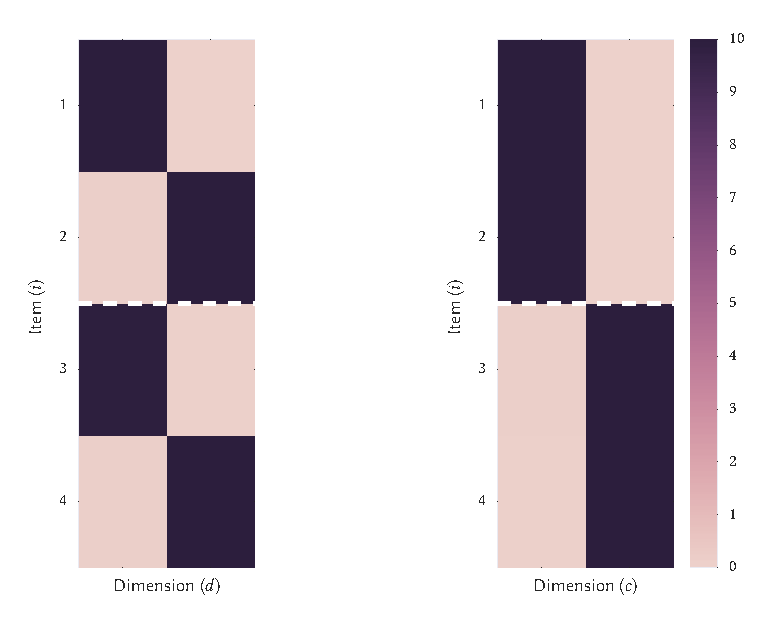
\includegraphics[height=6cm]{fldc_toy_example_mixed_weights}
  \caption{Diversity (left) and coherence weights (right) for FLDC model in example \ref{sec:fldc-toy}. The dotted line divides the paired items.}
  \label{fig:fldc-toy-mixed-weights}
\end{figure}


\section{Featurized model: FFLDC}

A important characteristic of the FLDC and FLID models is that they are agnostic to the type of items in the ground set, which allows its application to a wide range of problems without prior knowledge. However the downside is that the model has no capability to make use of the information about the items, if available, to improve the modeling of the data. Moreover, if a new item, which may be similar to previous items, is added to the set there is no way to generalize the existing knowledge about similar items to it.

In order to solve these problems, a further extension to the model is proposed. Firstly, the information about each item ($i \in V$) is represented as a vector $\mathbf{x}_{i} \in \mathbb{R}^{M}$. This vector represents the prior information about the items, e.g. for venues one feature could be its aggregated rating while another indicates whether it is indoors or outdoors.

Then, the utility vector $\mathbf{u}$ and weight matrices $\mathbf{W}^{D}, \mathbf{W}^{C}$ are decomposed to include the feature matrix $X \in \mathbb{R}^{|V| \times M}$ as follows:

\begin{align}
  \mathbf{u} &= \mathbf{Xa} \\
  \mathbf{W}^{D} &= \mathbf{XD} \\
  \mathbf{W}^{C} &= \mathbf{XC}
\end{align} 

Where $a \in \mathbb{R}^{M}$ represents the contribution of each feature to the total utility of an item, whilist $\mathbf{D} \in \mathbb{R}^{M \times L}$ and $\mathbf{C} \in \mathbb{R}^{M \times K}$ encode the contribution of each feature to each latent diversity and coherence dimension, respectively. The intuition behind this factorization is that the information about the items can enhance the latent representations, hence producing a richer model.

The extended model will be reffered to as Featurized Facility Location Diversity and Coherence (FFLDC) and its probability distribution is:

\begin{align}
  \tag{FFLDC}
  P(S) &= \frac{1}{Z}\exp{\left(\sum_{i \in S}{\mathbf{X}_{i,*}\mathbf{a}} + fdiv(S) + fcoh(S)\right)} \\
  fdiv(S) &= \sum_{d=1}^{L}{\left(\max_{i \in S}{\mathbf{X}_{i,*}\mathbf{D}_{*,d}} - \sum_{i \in S}{\mathbf{X}_{i,*}\mathbf{D}_{*,d}}\right)} \\
  fcoh(S) &= \sum_{c=1}^{K}{\left(\sum_{i \in S}{\mathbf{X}_{i,*}\mathbf{C}_{*,c}} - \max_{i \in S}{\mathbf{X}_{i,*}\mathbf{C}_{*,c}}\right)}
  \label{eq:ffldc}
\end{align}

\begin{remark}
  If $X = \mathcal{I}$, then FFLDC is equivalent to FLDC.
\end{remark}

The use of features also allows the extension of the model to previously unknown items, hence solving the aforementioned problem of generalization. This is because the parameters of the model, i.e. $\mathbf{a}, \mathbf{D}, \mathbf{C}$, do not depend on the ground set $V$ but rather the space of features $\mathbb{R}^{M}$. If an item $j \notin V$ is considered, a model learned on only items in $V$ can immediately be applied to the new set $V \cup \{j\}$, contrary to the case of FLID or FLDC where it would require adding a new row to the weight matrices and learning its components.

\subsection{Example: Rated locations}

\section{NCE learning}

Here goes a description of the objective function, what NCE is, guarantees. Also briefly describe SGD.

\subsection{Adagrad}

Describe the addition of Adagrad, and mention that it will be useful later.

\subsection{Learning FLID}

Short summary from what's on the AISTATS paper, show the gradient.

Show the results from learning the synthetic dataset from section \ref{sec:flid-toy}.

\subsection{Learning FLDC}

Add the gradient term for the coherence term.

Show the results from learning the synthetic dataset from section \ref{sec:fldc-toy}.

\subsection{Learning FFLDC}

Derive the gradients with features, show that the are the same as FLDC with X = I.

Show the results from learning the synthetic dataset from section \ref{sec:ffldc-toy}.

\subsection{Hyper-parameter sensitivity}

Use the synthetic datasets to show the effect of the following parameters:

\begin{itemize}
  \item Number of iterations
  \item Noise size
  \item Step size (with/without adagrad)
\end{itemize}

